\subsection{BÀI TẬP TRẮC NGHIỆM}
\Opensolutionfile{ans}[ans/ans0D6-B3]
\begin{ex}%[0D4B5]
	Biểu thức nào sau đây là một tam thức bậc hai đối với $x$?
	\choice
	{\True $f(x)=2x^2-\sqrt{3}$}
	{$f(x)=2x-1$}
	{$f(x)=\dfrac{x^2-1}{x}$}
	{$f(x)=\dfrac{x^2-x+1}{x+2}$}
	\loigiai{
	}
\end{ex}

\begin{ex}%[0D4B5]
	\immini{
		Cho hình vẽ bên, biết $f(x)=ax^2+bx+c$ và $\Delta=b^2-4ac$. Xác định dấu của $a$ và $\Delta$.
		\haicot
		{\True $a>0,\;\Delta <0$}
		{$a<0,\;\Delta <0$}
		{$a>0,\;\Delta >0$}
		{$a>0,\;\Delta =0$}}
	{
		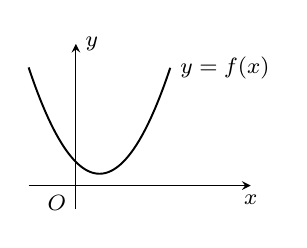
\begin{tikzpicture}[smooth,samples=300,scale=0.6,>=stealth,font=\footnotesize]
			\draw[->] (-1,0)--(3.7,0) node[below]{$x$};
			\draw[->] (0,-0.5)--(0,3) node[right]{$y$};
			\draw (0,0) node[below left]{$O$};
			\draw[line width=0.7pt,domain=-1:2] plot(\x,{(\x)^2-\x +0.5})node[right]{$y=f(x)$};
		\end{tikzpicture}
	}
	\loigiai{
		Từ hình vẽ suy ra hệ số $a>0$ và $\Delta <0$ (vô nghiệm).
	}
\end{ex}

\begin{ex}%[0D4B5]
	\immini{
		Cho hình vẽ bên, biết $f(x)=ax^2+bx+c$ và $\Delta=b^2-4ac$. Xác định dấu của $a$ và $\Delta$.
		\haicot
		{$a>0,\;\Delta <0$}
		{$a<0,\;\Delta <0$}
		{\True $a>0,\;\Delta >0$}
		{$a>0,\;\Delta =0$}}
	{
		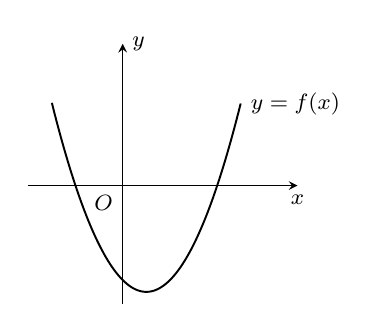
\begin{tikzpicture}[smooth,samples=300,scale=0.6,>=stealth,font=\footnotesize]
			\draw[->] (-2,0)--(3.7,0) node[below]{$x$};
			\draw[->] (0,-2.5)--(0,3) node[right]{$y$};
			\draw (0,0) node[below left]{$O$};
			\draw[line width=0.7pt,domain=-1.5:2.5] plot(\x,{(\x)^2-\x -2})node[right]{$y=f(x)$};
		\end{tikzpicture}
	}
	\loigiai{
		Từ hình vẽ suy ra hệ số $a>0$ và $\Delta >0$ (hai nghiệm phân biệt).
	}
\end{ex}

\begin{ex}%[0D4B5]
	\immini{
		Cho hình vẽ bên, biết $f(x)=ax^2+bx+c$ và $\Delta=b^2-4ac$. Xác định dấu của $a$ và $\Delta$.
		\haicot
		{\True $a<0,\;\Delta =0$}
		{$a<0,\;\Delta <0$}
		{$a>0,\;\Delta >0$}
		{$a>0,\;\Delta =0$}}
	{
		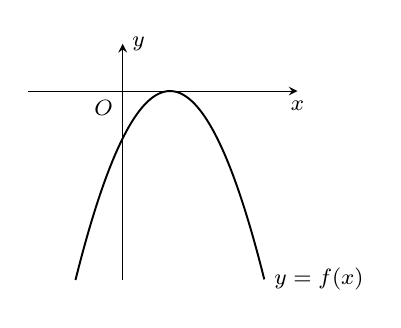
\begin{tikzpicture}[smooth,samples=300,scale=0.6,>=stealth,font=\footnotesize]
			\draw[->] (-2,0)--(3.7,0) node[below]{$x$};
			\draw[->] (0,-4)--(0,1) node[right]{$y$};
			\draw (0,0) node[below left]{$O$};
			\draw[line width=0.7pt,domain=-1:3] plot(\x,{-(\x-1)^2})node[right]{$y=f(x)$};
		\end{tikzpicture}
	}
	\loigiai{
		Từ hình vẽ suy ra hệ số $a<0$ và $\Delta =0$ (nghiệm kép).
	}
\end{ex}

\begin{ex}%[0D4B5]
	Tập hợp $T=(-1;3)$ là tập nghiệm của bất phương trình nào dưới đây?
	\choice{$-x^2+2x+3<0$}
	{$3x^2-2x-1>0$}
	{$x^2+2x-3<0$}
	{\True $x^2-2x-3<0$}
	\loigiai{
		Dùng MTCT, chọn chế độ giải bất phương trình bậc hai và kiểm tra từng phương án.
	}
\end{ex}

\begin{ex}%[0D4Y5-1]
	Bảng xét dấu nào sau đây là bảng xét dấu của biểu thức $f(x)=-x^2+14x-49$?
	\choice
	{
\begin{tikzpicture}[font=\footnotesize]
			\tkzTabInit[nocadre=false,lgt=1.3,espcl=1.8,deltacl=0.6]
			{$x$ /0.6,$f(x)$ /0.6}
			{$-\infty$,$7$,$+\infty$}
			\tkzTabLine{,+,$0$,+,}
	\end{tikzpicture}}
	{
\begin{tikzpicture}[font=\footnotesize]
			\tkzTabInit[nocadre=false,lgt=1.3,espcl=1.8,deltacl=0.6]
			{$x$ /0.6,$f(x)$ /0.6}
			{$-\infty$,$7$,$+\infty$}
			\tkzTabLine{,+,$0$,-,}
	\end{tikzpicture}}
	{\True 
\begin{tikzpicture}[font=\footnotesize]
			\tkzTabInit[nocadre=false,lgt=1.3,espcl=1.8,deltacl=0.6]
			{$x$ /0.6,$f(x)$ /0.6}
			{$-\infty$,$7$,$+\infty$}
			\tkzTabLine{,-,$0$,-,}
	\end{tikzpicture}}
	{
\begin{tikzpicture}[font=\footnotesize]
			\tkzTabInit[nocadre=false,lgt=1.3,espcl=1.8,deltacl=0.6]
			{$x$ /0.6,$f(x)$ /0.6}
			{$-\infty$,$7$,$+\infty$}
			\tkzTabLine{,-,$0$,+,}
	\end{tikzpicture}}
	\loigiai{
		\begin{itemize}
			\item [$\bullet$] $f(x)=-x^2+14x-49=0 \Leftrightarrow x=7$
			\item [$\bullet$] Bảng xét dấu
			\begin{center}
				
\begin{tikzpicture}[font=\footnotesize]
					\tkzTabInit[nocadre=false,lgt=1.3,espcl=1.8,deltacl=0.6]
					{$x$ /0.6,$f(x)$ /0.6}
					{$-\infty$,$7$,$+\infty$}
					\tkzTabLine{,-,$0$,-,}
				\end{tikzpicture}
			\end{center}
		\end{itemize}
	}
\end{ex}
\begin{ex}%[0D4B5-1]
	Bảng xét dấu sau là của biểu thức nào?
	\begin{center}
		
\begin{tikzpicture}
			\tikzset{t style/.style = {style = draw}}
			\tkzTabInit[lgt=1.5,espcl=2]
			{$x$ /0.7, $f(x)$ /0.8}
			{$-\infty$, $1$, $2$, $+\infty$}
			\tkzTabLine{ ,-,0,+,0,-, }
		\end{tikzpicture}
	\end{center}
	\choice
	{$f(x)=x^2+3x+2$}
	{\True $f(x)=-(x-1)(x-2)$}
	{$f(x)=-x^2-3x+2$}
	{$f(x)=x^2-3x+2$}
	\loigiai{
		Từ bảng xét dấu ta thấy $f(x)$ có hệ số $a<0$ và có 2 nghiệm phân biệt là $x=1$ và $x=2$ nên $f(x)=-(x-1)(x-2)$.}
\end{ex}

\begin{ex}%[0D4B5-2]
	Điều kiện cần và đủ để bất phương trình $ax^2+bx+c>0$, $\left(a \ne 0\right)$ vô nghiệm là gì?
	\choice
	{$\heva{&a<0 \\& \Delta >0.}$}
	{\True $\heva{&a<0 \\& \Delta \leq 0.}$}
	{$\heva{&a>0 \\& \Delta \leq 0.}$}
	{$\heva{&a<0 \\& \Delta <0.}$}
	\loigiai{
		Với  $a \ne 0$ thì 
		\allowdisplaybreaks
		\begin{eqnarray*}
			& ax^2+bx+c>0 \,\,\text{ vô nghiệm }& \Leftrightarrow   ax^2+bx+c\leq 0,\forall x\in \mathbb{R} \\
			& & \Leftrightarrow \heva{&a<0 \\& \Delta \leq 0.}
		\end{eqnarray*}
	}
\end{ex}

\begin{ex}%[0D4B5]
	Tìm tập nghiệm của bất phương trình $-5x^2+4x+12>0$.
	\choice{$\left(-\infty;-\dfrac{6}{5}\right)\cup \left(2;+\infty\right)$}
	{$\left(-2;\dfrac{6}{5}\right)$}
	{\True $\left(-\dfrac{6}{5};2\right)$}
	{$\left(-\infty;-2\right)\cup \left(\dfrac{6}{5};+\infty\right)$}
	\loigiai{
		Đặt $f(x)=-5x^2+4x+12$. Bảng xét dấu của $f(x)$ như sau
		\begin{center}
			
\begin{tikzpicture}
				\tikzset{t style/.style = {style = draw}}
				\tkzTabInit[lgt=1.5,espcl=2]
				{$x$ /0.7, $f(x)$ /0.8}
				{$-\infty$, $-\frac{6}{5}$, $2$, $+\infty$}
				\tkzTabLine{ ,-,0,+,0,-, }
			\end{tikzpicture}
		\end{center}
		Suy ra tập nghiệm là $\left(-\dfrac{6}{5};2\right)$.
	}
\end{ex}

\begin{ex}%[0D4B3]
	Tập xác định của hàm số $y=\sqrt{2x^2-5x-2}$ là 
	\choice
	{$\left(-\infty ; \dfrac{1}{2}\right]$}
	{$[2;+\infty) $}
	{\True $\left(-\infty ; \dfrac{1}{2}\right] \cup  [2;+\infty) $}
	{$\left[\dfrac{1}{2};2\right]$}
	\loigiai{
		Điều kiện xác định $2x^2-5x-2\ge 0$. Giải bất phương trình này ta được $x\le \dfrac{1}{2}$ hoặc $x \ge 2$.\\
		Vậy tập xác định là $\left(-\infty ; \dfrac{1}{2}\right] \cup  [2;+\infty) $.
	}
\end{ex}


\begin{ex}%[0D4B5]
	Bất phương trình nào dưới đây có tập nghiệm là $\mathbb{R}$? 
	\choice{$x^2+5x-7<0$}
	{\True $-x^2+x-5<0$}
	{$x^2-4x+4>0$}
	{$-2x^2+9x-13>0$}
	\loigiai{
		Dùng MTCT, chọn chế độ giải bất phương trình bậc hai và kiểm tra các phương án.
	}
\end{ex}

\begin{ex}%[0D4B3]
	Tam thức bậc hai $x^2-5x-6$ luôn dương khi
	\choice
	{\True $x<-1$ hoặc $x>6$}
	{$-1<x<6$}
	{$x\le -1$ hoặc $x\ge 6$}
	{$-1\le x\le 6$}
	\loigiai{
		Ta có $x^2-5x-6>0 \Leftrightarrow x<-1$ hoặc $x>6$.
	}
\end{ex}
\begin{ex}%[0D4B3]
	Tam thức bậc hai $-x^2+5x-4$ không âm khi
	\choice
	{ $x<1$ hoặc $x>4$}
	{$1<x<4$}
	{$x\le 1$ hoặc $x\ge 4$}
	{\True $1\le x\le 4$}
	\loigiai{
		Ta có $-x^2+5x-4 \ge 0 \Leftrightarrow 1\le x\le 4$.
	}
\end{ex}


\begin{ex}%[0D4K3]   
	Có bao nhiêu số nguyên $x$ để biểu thức $f(x)=(3x^2+x-2)^2-(x^2-x-7)^2$ luôn âm?
	\choice
	{$1$}
	{ $0$}
	{$2$}
	{\True$3$}
	\loigiai{
		Biến đổi 
		$$f(x)=(3x^2+x-2)^2-(x^2-x-7)^2=(4x^2-9)(2x^2+2x+5)$$
		Bảng xét dấu của $f(x)$ như sau
		\begin{center}
			
\begin{tikzpicture}
				\tikzset{t style/.style = {style = draw}}
				\tkzTabInit[lgt=1.5,espcl=2]
				{$x$ /0.7, $f(x)$ /0.8}
				{$-\infty$, $-\frac{3}{2}$, $\frac{3}{2}$, $+\infty$}
				\tkzTabLine{ ,+,0,-,0,+, }
			\end{tikzpicture}
		\end{center}
		Suy ra $f(x)<0 \Leftrightarrow x \in \left(-\dfrac{3}{2};\dfrac{3}{2} \right)$.\\
		Tập nghiệm này có các số nguyên sau: $-1$, $0$, $1$.
	}
\end{ex}

\begin{ex}%[0D4B5]
	Gọi $S$ là tập hợp nghiệm nguyên của bất phương trình $x^2-x-6 \leq 0$. Hãy chọn câu đúng.
	\choice
	{$S\subset \left(-2;3\right)$}
	{$S = \left(-2;3\right)$}
	{$S = \left(-2;3\right]$}
	{\True $S\subset \left(-3;4\right)$}
	\loigiai{
		Xét $$x^2-x-6 \leq 0 \Leftrightarrow -2 \le x \le 3.$$
		Suy ra tập $S=[-2;3]\subset \left(-3;4\right)$.
	}
\end{ex}

\begin{ex}
	\immini{Cho hàm số $f(x)=ax^2+bx+c$ có đồ thị như hình bên. Tìm tập nghiệm của bất phương trình $ax^2+bx+c \le 0$.
		\choice
		{ $(-\infty;0)\cup (2;+\infty)$}
		{\True $[0;2]$ }
		{ $(-\infty;0]\cup [2;+\infty)$}
		{$(0;2)$}}{\hspace{1cm}
		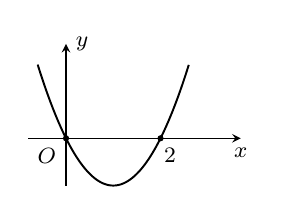
\begin{tikzpicture}[smooth,samples=300,scale=0.6,>=stealth,font=\footnotesize]
			\draw[->] (-0.8,0)--(3.7,0) node[below]{$x$};
			\draw[->] (0,-1)--(0,2) node[right]{$y$};
			\draw (0,0) node[below left]{$O$};
			\draw[line width=0.7pt,domain=-0.6:2.6] plot(\x,{(\x)^2-2*(\x)});
			\draw[fill=black] (2,0) circle(1.5pt) (0,0) circle(1.5pt);
			\node[below] at (2.2,0) {$2$};
	\end{tikzpicture}}
	\loigiai{
		$ax^2+bx+c \le 0$ tương ứng với phần đồ thị nằm phía dưới hoặc "chạm " $Ox$.\\ Từ hình vẽ, ta được $ax^2+bx+c \le 0 \Leftrightarrow 0 \le x \le 2$.
	}
\end{ex}

\begin{ex}
	\immini{Cho hàm số $f(x)=ax^2+bx+c$ có đồ thị như hình bên. Tìm tập nghiệm của bất phương trình $ax^2+bx+c \ge 0$.
		\choice
		{ $(-\infty;-2)\cup (1;+\infty)$}
		{ $(-\infty;-2]\cup [1;+\infty)$}
		{\True $[-2;1]$ }
		{$(0;2)$}}{\hspace{1cm}
		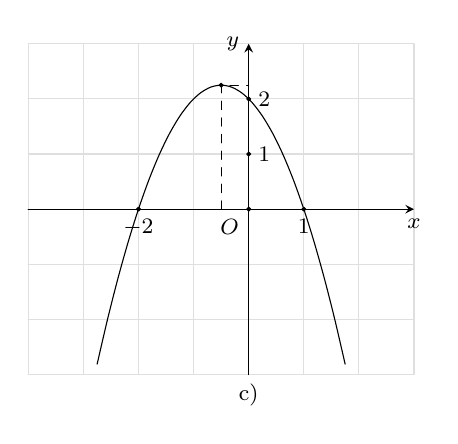
\begin{tikzpicture}[scale=.7, font=\footnotesize, line join=round, line cap=round, >=stealth]
			\draw[gray!50,opacity=.5](-4,-3)grid(3,3);
			\draw[->](-4,0)--(0,0)node[below left]{$O$}--(3,0)node[below]{$x$};
			\draw[->](0,-3)--(0,3)node[left]{$y$};
			\draw[smooth,domain=-2.75:1.75]plot(\x,{-(\x)^2-(\x)+2});
			\draw (0,-3)node[below]{c)};
			\draw(0,1)node[right]{$1$};
			\draw(0,2)node[right]{$2$};
			\draw(-2,0)node[below]{$-2$};
			\draw(1,0)node[below]{$1$};
			\draw[dashed](-0.5,0)--(-1/2,2.25)--(0,2.25);
			\foreach \x in {-2,0,1}\draw[fill](\x,0)circle(1pt);
			\foreach \x in {1,2}\draw[fill](0,\x)circle(1pt);
			\draw[fill](-1/2,2.25)circle(1pt);
			
	\end{tikzpicture}}
	\loigiai{
		$ax^2+bx+c \le 0$ tương ứng với phần đồ thị nằm phía trên hoặc "chạm " $Ox$.\\ Từ hình vẽ, ta được $ax^2+bx+c \ge 0 \Leftrightarrow -2 \le x \le 1$.
	}
\end{ex}

\begin{ex}
	\immini{Cho hàm số $f(x)=ax^2+bx+c$ có đồ thị như hình bên. Tìm tập nghiệm của bất phương trình $ax^2+bx+c \ge  3$.
		\haicot
		{ $[3;+\infty)$}
		{\True $[1;3]$ }
		{ $[0;4]$}
		{$[0;2]$}}{\hspace{1cm}
		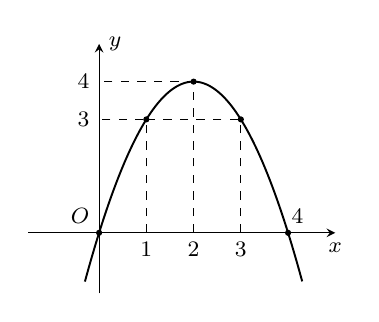
\begin{tikzpicture}[smooth,samples=300,scale=0.6,y=0.8cm,>=stealth,font=\footnotesize]
			\draw[->] (-1.5,0)--(5,0) node[below]{$x$};
			\draw[->] (0,-1.6)--(0,5) node[right]{$y$};
			\draw (0,0) node[above left]{$O$};
			\draw[line width=0.7pt,domain=-0.3:4.3] plot(\x,{-(\x)^2+4*(\x)});
			\draw[fill=black] (4,0) circle(1.5pt) (0,0) circle(1.5pt) (2,4) circle(1.5pt) (1,3) circle(1.5pt) (3,3) circle(1.5pt);
			\draw[dashed] (2,0)node[below]{$2$}--(2,4)--(0,4)node[left]{$4$}
			(1,0)node[below]{$1$}--(1,3)--(0,3)node[left]{$3$}
			(3,0)node[below]{$3$}--(3,3)--(1,3);
			\node[above] at (4.2,0) {$4$};
	\end{tikzpicture}}
	\loigiai{
		$ax^2+bx+c \ge 3$ tương ứng với phần đồ thị nằm phía trên hoặc "chạm " $y=3$.\\
		Từ hình vẽ, ta được $ax^2+bx+c \ge 0 \Leftrightarrow 1 \le x \le 3$.
	}
\end{ex}

\begin{ex}%[0D4B5-3]
	Cho $f(x)$, $g(x)$ là các hàm số xác định trên $\mathbb{R}$, có bảng xét dấu như sau
	\begin{center}
		
\begin{tikzpicture}
			\tkzTabInit[nocadre=false,lgt=1.5,espcl=2.5,deltacl=0.6] %phần bắt buộc
			{$x$/0.6, $f(x)$/0.6, $g(x)$/0.6} %phần bắt buộc
			{$-\infty$, $1$, $2$, $3$, $+\infty$} % hàng 1 cột 2
			\tkzTabLine{,+,z,-,t,-,z,+,}
			\tkzTabLine{,-,t,-,z,+,t,+,}
		\end{tikzpicture}
	\end{center}
	Khi đó tập nghiệm của bất phương trình $\dfrac{f(x)}{g(x)}\geq 0$ là
	\choice
	{$[1;2]$}
	{$[1;2)\cup (3;+\infty)$}
	{\True $[1;2)\cup [3;+\infty)$}
	{$[1;2]\cup (3;+\infty)$}
	\loigiai
	{
		Ta có bảng xét dấu của $\dfrac{f(x)}{g(x)}$ như sau
		\begin{center}
			
\begin{tikzpicture}
				\tkzTabInit[nocadre=false,lgt=1.5,espcl=2.5,deltacl=0.6] %phần bắt buộc
				{$x$/0.6, $f(x)$/0.6, $g(x)$/0.6, $\dfrac{f(x)}{g(x)}$/1.2} %phần bắt buộc
				{$-\infty$, $1$, $2$, $3$, $+\infty$} % hàng 1 cột 2
				\tkzTabLine{,+,z,-,t,-,z,+,}
				\tkzTabLine{,-,t,-,z,+,t,+,}
				\tkzTabLine{,-,z,+,d,-,z,+,}
			\end{tikzpicture}
		\end{center}
		Vậy tập nghiệm của bất phương trình $\dfrac{f(x)}{g(x)} \geq 0$ là $S=[1;2)\cup [3;+\infty)$.
	}
\end{ex}

\begin{ex}%[0D4K5]
	Có tất cả bao nhiêu giá trị nguyên của tham số $m$ để tam thức bậc hai $f(x)=-2x^2-\left(m+2\right)x+m^2-m-1$ luôn âm trên $\mathbb{R}$?
	\choice
	{$4$}
	{$3$}
	{$2$}
	{\True $1$}
	\loigiai{
		Tam thức bậc hai $f(x)$ có $a=-2<0$ nên 
		\begin{eqnarray*}
			\allowdisplaybreaks
			f(x)<0,\, \forall x \in \mathbb{R}
			&\Leftrightarrow&\Delta <0 \Leftrightarrow (m+2)^2+8(m^2-m-1)<0\\
			&\Leftrightarrow& 9m^2-4m-4<0 \\
			&\Leftrightarrow& \dfrac{2-2\sqrt{10}}{9}<m<\dfrac{2+2\sqrt{10}}{9}
		\end{eqnarray*}
		Các số nguyên thỏa điều kiện trên là $m=0$.
	}
\end{ex}

\begin{ex}%[0D4K5-2]
	Tìm tất cả giá trị thực của tham số $m$ để $-2x^2+(m+2)x+m-4 <0$ với mọi $x \in \mathbb{R}$. 
	\choice
	{$m<-14$ hoặc $m>2$}
	{$-14\le m\le 2$}
	{$-2<m<14$}
	{\True $-14<m<2$}
	\loigiai
	{
		Tam thức $f(x)$ có $a=-2<0$. Do đó
		\allowdisplaybreaks
		\begin{eqnarray*}
			f(x)<0,\forall x \Leftrightarrow (m+2)^2+8(m-4)<0 \Leftrightarrow m^2+12m-28\leq 0 \Leftrightarrow -14<m<2.
		\end{eqnarray*}
		Vậy $-14<m<2$ là các giá trị cần tìm.
	}
\end{ex}

\begin{ex}%[0D4T5-2]
	\immini{Xét một hình vuông lớn có kích thước $20 \times 20$. Từ hình vuông lớn, người ta cắt ra một hình vuông nhỏ như hình bên (\textit{các đỉnh hình vuông nhỏ nằm trên cạnh hình vuông lớn}). Tìm tập hợp các giá trị của $x$ để diện tích hình vuông nhỏ không vượt quá $208$.
		\haicot
		{\True $8 \leq x \leq 12$}
		{$6 \leq x \leq 14$}
		{$12 \leq x \leq 14$}
		{$12 \leq x \leq 18$}	
	}{\hspace{1cm}\begin{tikzpicture}[scale=1, line join = round, line cap = round]
			\tikzset{label style/.style={font=\footnotesize}}
			\tkzDefPoints{0/0/B,2/2/O}
			\tkzDefPointBy[rotation=center O angle -90](B)
			\tkzGetPoint{A}
			\tkzDefPointBy[rotation=center O angle 180](B)
			\tkzGetPoint{D}
			\tkzDefPointBy[rotation=center O angle 90](B)
			\tkzGetPoint{C}
			\tkzDefPointBy[homothety=center A ratio 0.3](D)
			\tkzGetPoint{E}
			\tkzDefPointBy[rotation=center O angle -90](E)
			\tkzGetPoint{F}
			\tkzDefPointBy[rotation=center O angle 180](E)
			\tkzGetPoint{G}
			\tkzDefPointBy[rotation=center O angle 90](E)
			\tkzGetPoint{H}
			\tkzDrawPolygon[color=black](A,B,C,D)
			\tkzDrawPolygon[color=magenta](E,F,G,H)
			\tkzDefPointBy[homothety=center B ratio 1.05](A)
			\tkzGetPoint{M}
			\tkzDefPointBy[homothety=center B ratio 1.05](C)
			\tkzGetPoint{P}
			\tkzDefPointBy[translation=from A to E](M)
			\tkzGetPoint{N}
			\tkzDefPointBy[translation=from C to D](P)
			\tkzGetPoint{Q}
			%\tkzLabelPoints[below](A,B,C,D,E,F,G,H)
			%\tkzFillPolygon[pattern=dots,pattern color=magenta](A,B,C,D)
			\tkzFillPolygon[pattern=dots,pattern color=green](E,F,G,H)
			\tkzDrawSegments[<->,above](M,N P,Q)
			\tkzLabelSegment[above](M,N){$x\;\mathrm{cm}$}
			\tkzLabelSegment[right](P,Q){$20\;\mathrm{cm}$}
			%\tkzMarkAngle[mark=|](C,A,B)
	\end{tikzpicture}}
	\loigiai{
		\immini{
			Gọi $E,F,G,H$ là bốn đỉnh của viên gạch hình vuông nội tiếp trong hình vuông $ABCD$ có cạnh $20$ cm như hình vẽ\\
			Ta có cạnh viên gạch là 
			$$EF=\sqrt{x^2+(20-x)^2}=\sqrt{2x^2-40x+400}.$$
			Diện tích của viên gạch là
			$$EF^2=2x^2-40x+400.$$
			Theo đề ta có diện tích viên gạch không vượt quá $208$ cm$^2$, suy ra
			$$2x^2-40x+400 \leq 208 \Leftrightarrow 2x^2-40x+192 \leq 0
			\Leftrightarrow 8 \leq x \leq 12.$$}
		{\hspace{1cm}\begin{tikzpicture}[scale=1, line join = round, line cap = round]
				\tikzset{label style/.style={font=\footnotesize}}
				\tkzDefPoints{0/0/B,2/2/O}
				\tkzDefPointBy[rotation=center O angle -90](B)
				\tkzGetPoint{A}
				\tkzDefPointBy[rotation=center O angle 180](B)
				\tkzGetPoint{D}
				\tkzDefPointBy[rotation=center O angle 90](B)
				\tkzGetPoint{C}
				\tkzDefPointBy[homothety=center A ratio 0.3](D)
				\tkzGetPoint{E}
				\tkzDefPointBy[rotation=center O angle -90](E)
				\tkzGetPoint{F}
				\tkzDefPointBy[rotation=center O angle 180](E)
				\tkzGetPoint{G}
				\tkzDefPointBy[rotation=center O angle 90](E)
				\tkzGetPoint{H}
				\tkzDrawPolygon[color=magenta](A,B,C,D)
				\tkzDrawPolygon[color=magenta](E,F,G,H)
				\tkzDefPointBy[homothety=center B ratio 1.05](A)
				\tkzGetPoint{M}
				\tkzDefPointBy[homothety=center B ratio 1.05](C)
				\tkzGetPoint{P}
				\tkzDefPointBy[translation=from A to E](M)
				\tkzGetPoint{N}
				\tkzDefPointBy[translation=from C to D](P)
				\tkzGetPoint{Q}
				\tkzLabelPoints[left](A,B,H)
				\tkzLabelPoints[right](C,D,F)
				\tkzLabelPoints[above](E)
				\tkzLabelPoints[below](G)
				\tkzFillPolygon[pattern=dots,pattern color=magenta](A,B,C,D)
				\tkzFillPolygon[pattern=dots,pattern color=green](E,F,G,H)
				\tkzDrawPoints(A,B,C,D,E,F,G,H)
				\tkzLabelSegment[above](A,E){$x$}
				\tkzLabelSegment[above](E,D){$20-x$}
				%\tkzMarkAngle[mark=|](C,A,B)
		\end{tikzpicture}}		
	}
\end{ex}

\begin{ex}
	Kim muôn trồng một vườn hoa trên mảnh đât hình chữ nhật và làm hàng rào bao quanh. Kim chỉ có đủ vật liệu để làm $30 \mathrm{~m}$ hàng rào nhưng muốn diện tích vườn hoa ít nhất là $50 \mathrm{~m}^{2}$. Hỏi chiều rộng của vườn hoa nằm trong khoảng nào?
	\choice
	{$[8 ; 12]$}
	{$[3 ; 7]$}
	{\True $[5 ; 10]$}
	{$[10 ; 15]$}
	\loigiai{
	Gọi $x(\mathrm{~m})$ là chiều rộng của mảnh vườn.
	Chiều dài của mảnh vườn là $(15-x)(\mathrm{m})$.
	Diện tích mảnh vườn là $x(15-x) \geq 50$, suy ra $5 \leq x \leq 10$.
	Vậy chiều rộng mảnh vườn nằm trong đoạn $[5 ; 10]$ (mét).}
\end{ex}

\begin{ex}
	Một quả bóng được ném thẳng lên từ độ cao $1,6 \mathrm{~m}$ so với mặt đất với vận tốc $10 \mathrm{~m} / \mathrm{s}$. Độ cao của bóng so với mặt đất (tính bằng mét) sau $t$ giây được cho bởi hàm số $h(t)=-4,9 t^{2}+10t+1,6$. Hỏi bóng ở độ cao trên $5 \mathrm{~m}$ trong khoảng thời gian bao lâu? Làm tròn kết quả đến hàng phần trăm.
	\choice
	{1,5 giây}
	{0,98 giây}
	{\True 1,18 giây}
	{1,35 giây}
	\loigiai{
		Giải bất phương trình $-4,9 t^{2}+10 t+1,6>5$.
		Ta kết luận được bóng ở độ cao trên $5 \mathrm{~m}$ trong thời gian khoảng 1,18 giây.
	}
\end{ex}

\begin{ex}
	Mặt căt ngang của mặt đường thường có dạng hình parabol đê nước mưa dê dàng thoát sang hai bên. Mặt cắt ngang của một con đường được mô tả bằng hàm số $y=-0,006 x^{2}$ với gốc toạ độ đặt tại tim đường và đơn vị đo là mét như hình bên dưới. 
	\begin{center}
		\begin{tikzpicture}[smooth,samples=300,scale=0.8,>=stealth,y=1.5cm,font=\footnotesize]
			\draw[->] (-8,0)--(8,0) node[below]{$x$};
			\draw[->] (0,-0.5)--(0,1) node[right]{$y$};
			\draw (0,0) node[above left]{$O$};
			\draw[line width=2pt,domain=-7:7,gray] plot(\x,{-0.006*(\x)^2});
			\draw[fill=black] (-7,-0.294) circle(2pt) (7,-0.294) circle(2pt);
			\draw[] (-7,-0.294)node[below]{lề đường}--(7,-0.294)node[below]{lề đường};
			\fill[pattern = dots,smooth] (-7,-0.294)--plot[domain=-7:7](\x,{-0.006*(\x)^2})--(7,-0.294)--cycle;
			%\node[right] at (2,2.4) {$2$};
		\end{tikzpicture}
	\end{center}
	Với chiều rộng của đường như thế nào thì tim đường cao hơn lề đường không quá $15 \mathrm{~cm}$ ?
	\choice
	{12 m}
	{8 m}
	{\True 10 m}
	{15 m}
	\loigiai{
		Giải bất phương trinh $-0,006 x^{2} \geq-0,15$, suy ra $-5 \leq x \leq 5$.
		Vậy chiều rộng của đường không vượt quá $5-(-5)=10(\mathrm{~m})$.
	}
\end{ex}


\centerline{\textbf{---HẾT---}}
\Closesolutionfile{ans}